
\documentclass{beamer}

\usepackage{algpseudocode, color, colortbl, listings, MnSymbol}

\usepackage{hyperref}
\hypersetup{
    colorlinks=true,
    urlcolor=blue,
}

\usetheme{Montpellier}
\usecolortheme{rose}

% page numbers, from
% https://tex.stackexchange.com/questions/137022/how-to-insert-page-number-in-beamer-navigation-symbols
\expandafter\def\expandafter\insertshorttitle\expandafter{%
  \insertshorttitle\hfill%
  \insertframenumber\,/\,\inserttotalframenumber}

\definecolor{Gray}{gray}{0.8}
\newcolumntype{g}{>{\columncolor{Gray}}c}

\newcommand{\stanza}{ \\~\ }

\title{10. Computational Geometry}
\subtitle{CPSC 535 $\sim$ Spring 2019}
\author{Kevin A. Wortman}
\institute{ 
\includegraphics[height=2cm]{csuf-logo-cmyk} }
\date{April 22, 2019 \stanza

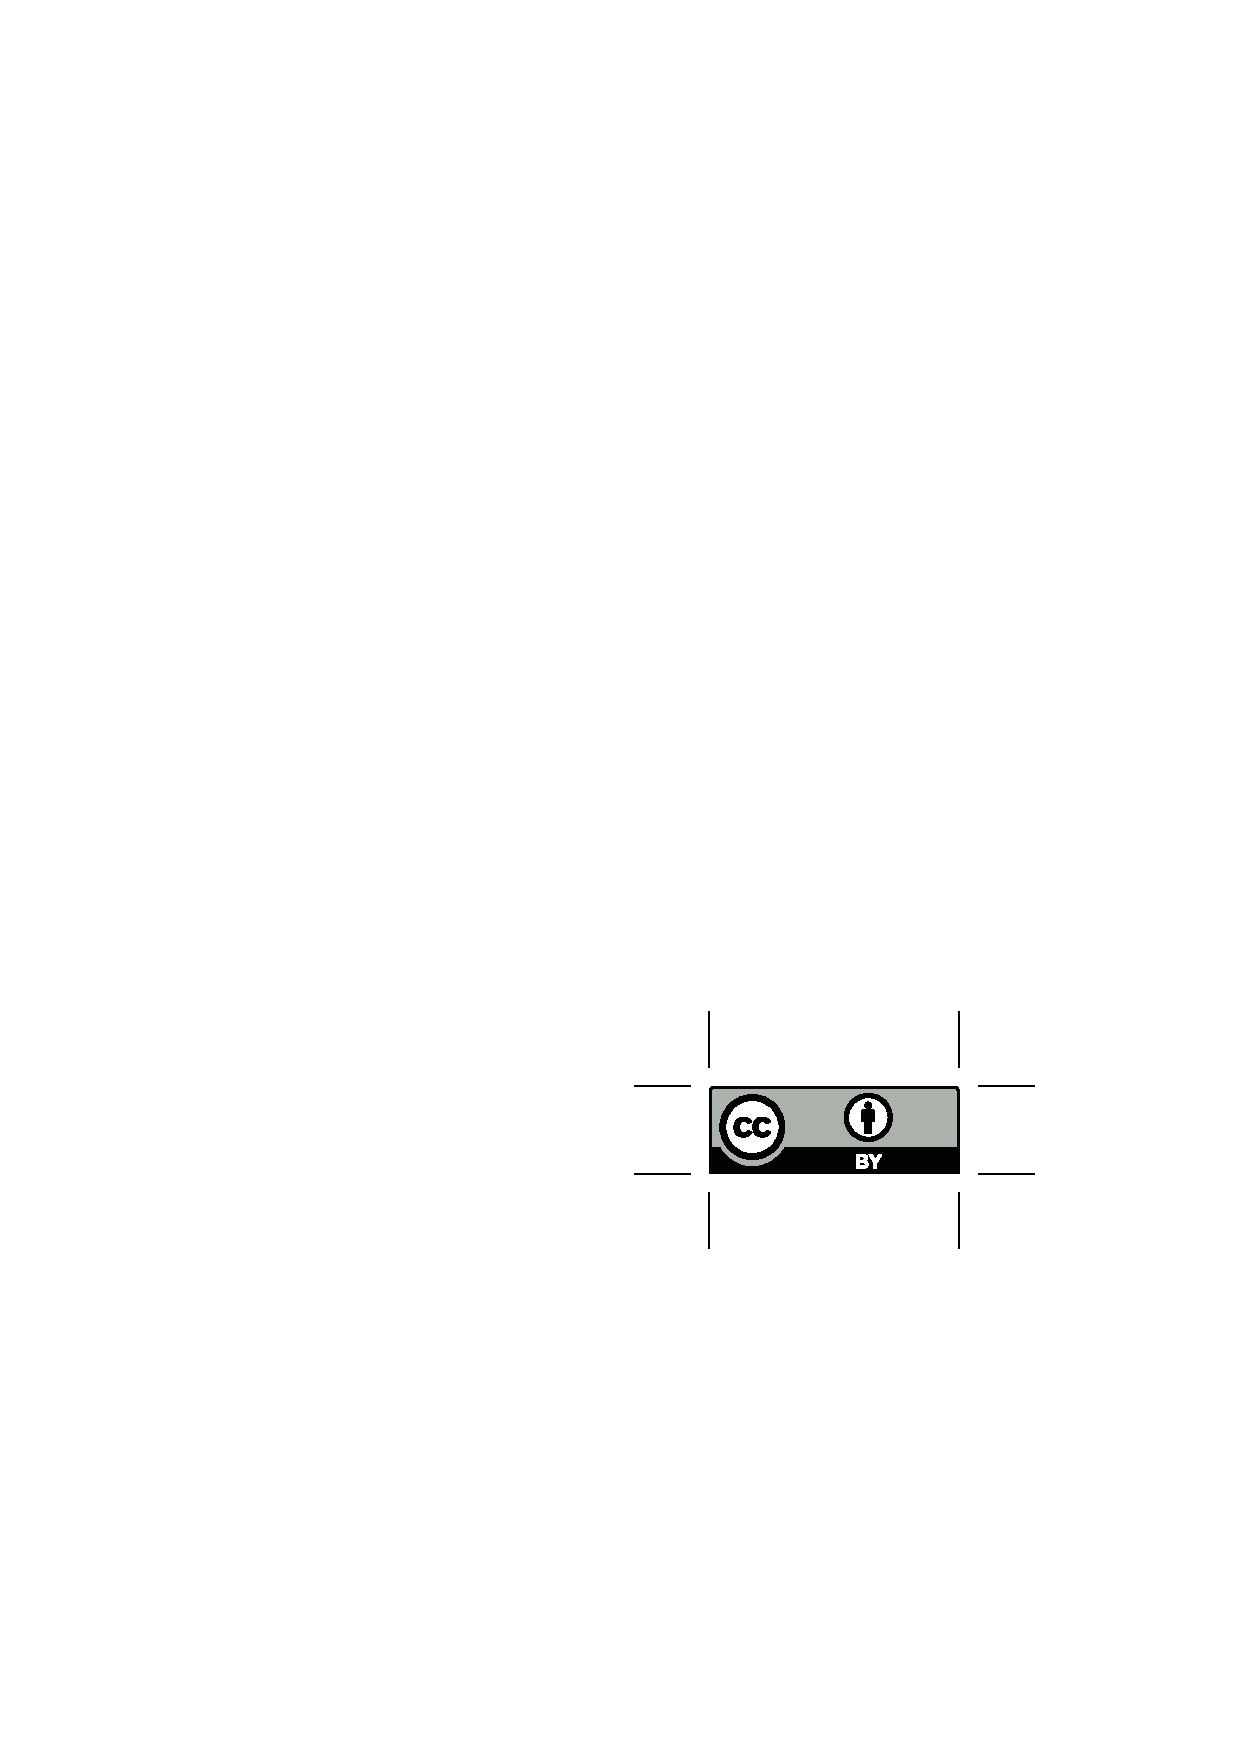
\includegraphics[height=14pt]{by} \\

{\tiny
This work is licensed under a
\href{http://creativecommons.org/licenses/by/4.0/}{Creative Commons Attribution 4.0 International License}.
}}

\begin{document}

\begin{frame}
  \titlepage
\end{frame}

\begin{frame} \frametitle{Big Idea: Generality versus Specialization}
Common sense: very general problems are harder to solve than specific problems.
\stanza

Mathematics:
\begin{itemize}
  \item Theorems are stated ``If $A$ then $B.$''
  \item $A$ the \emph{antecedent}, $B$ the \emph{consequent.}
  \item More constraints in $A$ means either $B$ is easier to prove; or
    we can prove a stronger version of $B$.
\end{itemize}
\end{frame}

\begin{frame} \frametitle{Example: Shortest Paths}

\emph{single source shortest paths problem} \\
 \textbf{input}: weighted graph $G=(V,E)$, start vertex $s \in V$ \\
 \textbf{output}: for each $v \in V,$ a shortest path from $s$ to $v$ \stanza

As stated: Bellman-Ford algorithm takes $\Theta(mn)$ time. \stanza

Constrain all edge weights to be non-negative \\
$\implies$ Dijkstra's algorithm takes only $\Theta(m + n \log n)$ time. \stanza

The constraint that weights are nonnegative makes the problem easier to solve
(negative cycles d.n.e.) so it admits a faster algorithm.
\end{frame}

\begin{frame} \frametitle{Big Idea: Output Sensitive Algorithm}
  \begin{itemize}
    \item \textbf{input sensitive}: (time) efficiency is a function of the input
      e.g. size $n$, \# edges $m$, maximum word $W$
    \item \textbf{output sensitive}: efficiency is also a function of the
      \emph{output} e.g. \# items returned
    \item most relevant when the size of the output may or may not be a
      bottleneck
  \end{itemize}
\end{frame}

\begin{frame} \frametitle{Example: Matching Index Pairs}
\emph{matching index pairs problem} \\
\textbf{input}: sets $L[0..\ell], R[0..r]$ \\
\textbf{output}: each pair $(i, j)$ where $L[i]=R[j]$ \stanza

Let $k \equiv$ number of pairs in output \stanza

Nested for loops: $\Theta(\ell r)$, regardless of $k$ \stanza

Using a hash table:
\begin{itemize}
  \item $\Theta(\ell + r + k)$
  \item $k \leq \ell r;$ hash alg. is same speed for large $k$
  \item but is much faster for small $k$
  \item improvement when small $k$ is likely or guaranteed
\end{itemize}
\end{frame}

\begin{frame} \frametitle{Computational Geometry}
\textbf{computational $X$}: interdisciplinary study of computer science with $X$ \\
(computational sociology/epidemiology/physics/finance/etc.) \stanza

computational geometry (CG): algorithms, data structures, asymptotic analysis, of
geometric objects: points, lines, circles, triangle meshes, etc. \stanza

Applications
\begin{itemize}
  \item computer graphics, user interfaces
  \item GIS, geographic databases
  \item scene reconstruction (e.g. LIDAR)
  \item business operations research (e.g. linear programming, aircraft control)
  \item manufacturing (e.g. feasibility of assembly, castings)
\end{itemize}
\end{frame}

\begin{frame} \frametitle{Putting the Geo in CG}
Some general algorithms can actually solve geometric problems efficiently, without
any awareness of the geometry. \stanza

\emph{bounding box problem} \\
\textbf{input}: set of 2D points $P=\{p_1, p_2, \ldots, p_n\}$ \\
\textbf{output}: points $tl=(x_l, y_t)$ and $rb=(x_r, y_b)$ such that the rectangle
with top-left corner $tl$ and bottom-right corner $rb$ contains $P$ \stanza

Na\"{i}ve, optimal algorithm: $x_l, y_t, x_r, y_b = $ min $x$, min $y$, max $x$,
max $y$ respectively; $\Theta(n)$ \stanza

Computational geometers are most interested when geometric properties matter.
\end{frame}

\begin{frame} \frametitle{Line Segment Predicates}
We can use arithmetic to answer any of the following predicates (questions)
about points $p_0, p_1, p_2, p_3$ in $\Theta(1)$ time:
\begin{enumerate}
  \item Is line segment $\overline{p_0 p_1}$ clockwise from $\overline{p_0 p_2}$
    around the common endpoint $p_0$?
  \item If we follow $\overline{p_0 p_1}$ and then $\overline{p_1 p_2}$, do we
    turn right or left?
  \item Do line segments $\overline{p_0 p_1}$ and $\overline{p_2 p_3}$
    intersect?
\end{enumerate}

$\implies$ We may use any of these in pseudocode.
\end{frame}

\begin{frame} \frametitle{Degeneracy and Non-Degeneracy Assumptions}
\textbf{degenerate} object: has the proper shape/type, but the values are a
  special case that betrays the spirit of the definition \stanza

\emph{Example:} triangle $\equiv$ three points $(p_1, p_2, p_3)$ \\
degenerate triangle: $p_1=p_2=p_3$; or $p_1, p_2, p_3$ colinear; etc. \stanza

\textbf{Non-degeneracy assumption}:
\begin{itemize}
  \item constraint that input to a CG algorithm is not degenerate in specific ways
  \item simplifies algorithm design
  \item assume that in practice, some combination of
  \begin{itemize}
    \item degeneracies do not occur
    \item input can be preprocessed to remove degeneracies
    \item implementer can modify algorithm to handle degeneracies
  \end{itemize}
\end{itemize}
\end{frame}

\begin{frame} \frametitle{Line Segment Intersection}
\emph{line segment intersection problem} \\
\textbf{input}: set of $n$ line segments
  $L=\{ ((x_1, y_1), (x_2, y_2)) : x_1, y_1, x_2, y_2 \in \mathbb{R} \}$ \\
\textbf{output}: some pair $\ell, \ell' \in L$ that intersect, or NIL if
  no segments in $L$ intersect \stanza

Non-degeneracy assumptions:
\begin{itemize}
  \item no segments are vertical
  \item no three segments intersect in a common point
\end{itemize}

Thought exercise: How realistic is this? How hard would it be to sanitize input
without affecting the output? \stanza

Baseline algorithm: nested for loops, $\Theta(n^2)$ time.
\end{frame}

\begin{frame} \frametitle{Sweep Algorithms}
A pattern in CG algorithms:
\begin{itemize}
  \item \emph{line sweep:} envision a line ``sweeping'' through the input
  \item e.g. a vertical line sweeping left-to-right
  \item helps us visualize a 2D situation as a 1D situation that changes over
    time
  \item like duality, doesn't actually change the problem, but might help us
    problem-solve
  \item generalizes to higher dimensions e.g. plane sweep in 3D, hyperplane sweep
    in any dimension
\end{itemize}
\end{frame}

\begin{frame} \frametitle{Geometric Insight}
\begin{itemize}
  \item Visualize vertical line sweeping left-to-right.
  \item Consider some segment $\ell$; at some point $\ell$'s left endpoint will strike
    the sweep line; then the common point will slide a bit as the sweep continues;
    then the sweep will move past the $\ell$'s right endpoint.
  \item These time steps are discrete \textbf{events} that matter; fast-forward
    past in-between moments.
  \item Consider the ordering of active line segments along the sweep line
    in top-to-bottom order.
  \item \emph{If two segments swap order between time events, then they must intersect.}
\end{itemize}
\end{frame}

\begin{frame} \frametitle{Line Segment Intersection Pseudocode}
\includegraphics[height=2.5in]{10-lines.png}
\end{frame}

\begin{frame} \frametitle{Non-Degeneracy Assumptions Revisited}
Algorithm assumes that
\[ \text{sweep line } \cap \text{ each line segment} \]
is only one point \\
$\implies$ require that no segment is vertical. \stanza

Algorithm assumes that intersecting segments only move \emph{one} step
in top-to-bottom order \\
$\implies$ require that 3+ segments may never intersect at the same point.
\end{frame}

\begin{frame} \frametitle{BST Operations Review}
create empty: $\Theta(1)$ \\
search, insert, delete: $\Theta(\log n)$ \stanza

Predecessor/successor query:
\begin{itemize}
  \item esoteric BST operation, yet still available in e.g. C++ STL
  \item given pointer to a node, find its inorder predecessor/successor
  \item can visualize as moving to the previous/next step in an Euler tour
    (sketch)
  \item $\Theta(\log n)$
\end{itemize}
\end{frame}

\begin{frame} \frametitle{Line Intersection Analysis}
  sort points: $\Theta(n log n)$ \stanza

  for loop: $2n \in \Theta(n)$ events \\
  body of loop involves $\Theta(1)$ BST operations \\
  $\implies$ $\Theta(\log n)$ time per iteration \stanza

  $\Theta(n \log n + n \log n) = \Theta(n \log n)$ total time \stanza

  Example of reduction to both sorting and BST operations.
\end{frame}

\begin{frame} \frametitle{Convex Hulls}
\emph{convex hull problem} \\
\textbf{input}: set of $n \geq 3$ points $Q$ \\
\textbf{output}: $CH(Q)$, the subset of $Q$ that is the set of vertices on
  the convex hull of $Q$ \stanza

Convex hull $\equiv$ convex polygon enclosing all of $Q$ \stanza

Applications
\begin{itemize}
  \item object intersection in raytracing, video games, GUIs
  \item drawing implicit regions in GIS
  \item finding farthest points
  \item component of other algorithms
\end{itemize}
\end{frame}

\begin{frame} \frametitle{Approaches to Convex Hulls}
Like the sorting problem, many algorithm patterns work for convex hulls,
and there is a rich literature of competitive algorithms. \stanza

\begin{itemize}
  \item Greedy pattern: line-sweep, update hull as we go
  \item Divide-and-conquer: divide $Q$ in half, compute convex hulls for each
    half, merge two convex hulls into one
  \item Iterative improvement: start with a superset of $CH(Q)$; refine by repeatedly eliminating
    a constant fraction of the points until only $CH(Q)$ remains
\end{itemize}
\end{frame}

\begin{frame} \frametitle{Graham Scan}

  (TODO)

\end{frame}

\begin{frame} \frametitle{Jarvis March}
Greedy heuristic: moving around the hull counter-clockwise, each step from one
  vertex to the next is \emph{the input point whose angle is shallowest} \stanza

Jarvis march
\begin{enumerate}
  \item Find the lowest and highest points in $Q$.
  \item (right chain)
  \item Starting from the lowest point, and until we reach the highest point:
    \begin{enumerate}
      \item Linear search $Q$ for the next point, minimizing the angle between
        the two points.
      \item Add the first point to $CH(Q)$ and move to the second point.
    \end{enumerate}
  \item (left chain) Starting from the highest point, repeat this process until we
    reach the lowest point.
  \item Return $CH(Q)$
\end{enumerate}
\end{frame}

\begin{frame} \frametitle{Jarvis March Analysis}
  Preprocessing to find points: $\Theta(n)$ \stanza

  Loops together iterate $h$ times, where $h \equiv $ number of points on the hull. \stanza

  The linear search inside the loop takes $\Theta(n)$ time. \stanza

  $\therefore$ $\Theta(nh)$ total time. \\
  Faster than Graham scan's $\Theta(n \log n)$ when $h \in o(\log n).$
\end{frame}

\end{document}
